Before conducting any kind of machine learning experiment there is a need to specify values of hyperparameters and coefficients that are required for proper functioning of the system. Table \ref{table:hyperparameters_linear} presents chosen values of each parameter that was needed to perform all experiments described in this chapter.
\begin{table}[ht]
    \caption{Values of hyperparameters required for colour-based segmentation.}
    \centering
    \begin{tabular}{|l|c|}
        \hline
        \rowcolor[HTML]{cecaca} 
        \textbf{Parameter name} & \textbf{Parameter value} \\ \hline
        Number of images (inputs) & 200 \\ \hline
        Number of states (outputs) & 3 \\ \hline
        Number of superpixels & 500 \\ \hline
        Training step & 0.0001 \\ \hline
        Regularisation factor & 1000 \\ \hline
        Number of training epochs & 5 \\ \hline
        Convergence tolerance & 0.1 \\ \hline
    \end{tabular}
    \label{table:hyperparameters_linear}
\end{table}

\subsection{Semantic segmentation on tricoloured image}

The first experiment of this part of the system was aimed to perform segmentation on a set of simple images composed of only red, green and blue regions as it has already been presented in \textit{section \ref{sec:linear_dataset}: \nameref{sec:linear_dataset}}. Every image was modelled with a factor graph containing two types of nodes: input, and output. Nodes of the first type contained information about properties of a given superpixel, which in this part of the system were three features representing three components of a superpixel colour. For this experiment the RGB colour space was chosen to model those features, hence, in a given image a feature vector of a superpixel can take only one of the three possible values $[255,0,0]$, $[0,255,0]$, and $[0,0,255]$. The goal of this experiment was to differentiate red, green, and blue regions, thus, the output nodes can also have one of the three possible values: label 0 for red superpixels, 1 for green, and 2 for blue ones. After the processes of feature extraction and factorisation are completed, the next step is parameter training by means of Stochastic Gradient Descent. In this process, eleven weights of the system were adjusted to match the training set of images that was already described. The goal was to learn such weights that the total energy of a factor graph for a given image would be minimised. Hence, for label 0 red component of colour should be promoted, thus having a small weight, for label 1 a green one, and for label 2 a blue colour component. For this experiment weights for the pairwise potential are not so important as there is no noise in training images. Table \ref{table:weights_linear_exp_1} shows values of weights after the training process was completed. It can be seen in the table that weights for the local potential match the expectations, hence, the training process was successful.
\npdecimalsign{.}
\nprounddigits{5}
\begin{table}[ht]
    \caption{Trained weights for segmentation of tricoloured images.}
    \centering
    \begin{tabular}{|
    >{\columncolor[HTML]{cecaca}}c|n{2}{6}|n{2}{6}|n{2}{6}|}
    \multicolumn{4}{c}{\cellcolor[HTML]{656565}{\color[HTML]{FFFFFF} \textit{local weights}}} \\ \hline
     & \multicolumn{1}{c|}{\cellcolor[HTML]{cecaca}red} & \multicolumn{1}{c|}{\cellcolor[HTML]{cecaca}green} & \multicolumn{1}{c|}{\cellcolor[HTML]{cecaca}blue} \\ \hline
    label 0 & -0.04148262363505202 & 0.02088709381110257 & 0.012204837263693908 \\ \hline
    label 1 & 0.02053515535187271 & -0.04250326661084058 & 0.013991170837388876 \\ \hline
    label 2 & 0.020947468283179317 & 0.02161617279973801 & -0.026196008101082784 \\ \hline
    \multicolumn{4}{c}{\cellcolor[HTML]{656565}{\color[HTML]{FFFFFF} \textit{pairwise weights}}} \\
    $y_i = y_j$ & -0.2191765937200767 &  &  \\ \hline
    $y_i \neq  y_j$ & 0.2191765937200767 &  &  \\ \hline
    \end{tabular}
     \label{table:weights_linear_exp_1}
\end{table}

Then, with a trained model an inference process for unknown images can be performed. Figure \ref{fig:linear_basic_result_exp1} depicts five sample test image together with their output labellings being a result of the inference process and a reference labelling. On all three types of images borders of superpixels were marked for the sake of better visualisation of the results.
\begin{figure}[!htb]
 \centering
    \begin{tabular}{ccc}
        \textit{sample image} & \textit{experimental result} & \textit{expected results} \\
       \fcolorbox{black}{white}{\includegraphics[width = 0.20\textwidth]{linear_no_noise/experiments/images/0.png}} &
        \fcolorbox{black}{white}{\includegraphics[width = 0.20\textwidth]{linear_no_noise/experiments/results/0.png}} &
        \fcolorbox{black}{white}{\includegraphics[width = 0.20\textwidth]{linear_no_noise/experiments/expected/0.png}} \\
        \fcolorbox{black}{white}{\includegraphics[width = 0.20\textwidth]{linear_no_noise/experiments/images/1.png}} &
        \fcolorbox{black}{white}{\includegraphics[width = 0.20\textwidth]{linear_no_noise/experiments/results/1.png}} &
        \fcolorbox{black}{white}{\includegraphics[width = 0.20\textwidth]{linear_no_noise/experiments/expected/1.png}} \\
        \fcolorbox{black}{white}{\includegraphics[width = 0.20\textwidth]{linear_no_noise/experiments/images/2.png}} &
        \fcolorbox{black}{white}{\includegraphics[width = 0.20\textwidth]{linear_no_noise/experiments/results/2.png}} &
        \fcolorbox{black}{white}{\includegraphics[width = 0.20\textwidth]{linear_no_noise/experiments/expected/2.png}} \\
        \fcolorbox{black}{white}{\includegraphics[width = 0.20\textwidth]{linear_no_noise/experiments/images/4.png}} &
        \fcolorbox{black}{white}{\includegraphics[width = 0.20\textwidth]{linear_no_noise/experiments/results/4.png}} &
        \fcolorbox{black}{white}{\includegraphics[width = 0.20\textwidth]{linear_no_noise/experiments/expected/4.png}} \\
        \fcolorbox{black}{white}{
\includegraphics[width = 0.20\textwidth]{linear_no_noise/experiments/images/6.png}} &
        \fcolorbox{black}{white}{
\includegraphics[width = 0.20\textwidth]{linear_no_noise/experiments/results/6.png}} &
        \fcolorbox{black}{white}{
\includegraphics[width = 0.20\textwidth]{linear_no_noise/experiments/expected/6.png}} \\
    \end{tabular}
    \caption{Experimental results of semantic image segmentation on sample tricoloured images.}
    \label{fig:linear_basic_result_exp1}
\end{figure}
Based on the presented images it can be stated that the semantic segmentation of test images was successful. As expected, each red shape was marked with label 0, shown on the resulting image in black colour. Similarly, all green and blue regions have a proper class assigned, which are label 1, painted in white and label 2 marked in grey, respectively.

The accuracy of the described segmentation method is presented in Table \ref{table:iou_linear_exp1}. For each label, Intersection over Union was computed based on the presented test set. The final accuracy of the method is expressed as mean Intersection over Union (mIoU), and for this experiment, the precision of results was equal to 100\%.
\begin{table}[ht]
\centering
\caption{Accuracy of segmentation for tricoloured images expressed in IoU for each class.}
\label{table:iou_linear_exp1}
    \begin{tabular}
    {|>{\columncolor[HTML]{cecaca}}c|c|c|c|>{\columncolor[HTML]{343434}}c|} 
    \hline
    \textit{class} & \cellcolor[HTML]{cecaca}label 0 & \cellcolor[HTML]{cecaca}label 1 & \cellcolor[HTML]{cecaca}label 2 & {\color[HTML]{FFFFFF} mIoU {[}\%{]}} \\ \hline 
    IoU {[}\%{]} & 100.00 & 100.00 & 100.00 & {\color[HTML]{FFFFFF} 100.00} \\ \hline
    \end{tabular}
\end{table}
 
\subsection{Semantic segmentation on multicoloured image}

The goal of the second experiment was exactly the same as in the first one, which is to perform semantic segmentation of images into three classes. However, in this experiment a training and a testing set were composed of multicoloured images. Instead of having only red, green and blue superpixels also shades of those colours were introduced. Moreover, in this experiment importance of the pairwise potential will be tested as there are some superpixels in the test images which colour is less similar to the respective basic colour, meaning red, green, or blue, than the colour of its neighbours. For such regions, pairwise potential should promote a situation in which this superpixel will take the same label as the adjacent superpixels. The procedure of segmentation is exactly the same as previously, however, in this experiment feature vectors are composed of continuous values representing a shade of a given superpixel colour component and not one of the two available values 0 or 255, as it was before.

Table \ref{table:weights_linear_exp2_1} shows the values of weights obtained by the process of parameter training. Once again, for label 0 the red component is smaller than the others, for label 1 the green component, and for label 3 the blue one, which is an expected behaviour. Pairwise weights are similar as in case of the first experiment.
\npdecimalsign{.}
\nprounddigits{5}
\begin{table}[!htb]
    \caption{Trained weights for segmentation of multicoloured images using RGB features.}
    \centering
    \begin{tabular}{|
    >{\columncolor[HTML]{cecaca}}c |n{2}{6}|n{2}{6}|n{2}{6}|}
    \multicolumn{4}{c}{\cellcolor[HTML]{656565}{\color[HTML]{FFFFFF} \textit{local weights}}} \\ \hline
     & \multicolumn{1}{c|}{\cellcolor[HTML]{cecaca}red} & \multicolumn{1}{c|}{\cellcolor[HTML]{cecaca}green} & \multicolumn{1}{c|}{\cellcolor[HTML]{cecaca}blue} \\ \hline
    label 0 & -0.01929696880558088 & 0.00967165632403644 & 0.014061761254553109 \\ \hline
    label 1 & 0.013121748946249215 & -0.013694388602578954 & 0.01513050683624383 \\ \hline
    label 2 & 0.00617521985933168 & 0.0040227322785425495 & -0.02919226809079693 \\ \hline
    \multicolumn{4}{c}{\cellcolor[HTML]{656565}{\color[HTML]{FFFFFF} \textit{pairwise weights}}} \\
    $y_i = y_j$ & -0.23531971785110614 &  &  \\ \hline
    $y_i \neq  y_j$ & 0.23531971785110614 &  &  \\ \hline
    \end{tabular}
     \label{table:weights_linear_exp2_1}
\end{table}

After parameter training is completed, with the use of the established weights an inference process can take place. Similarly as in the first experiment, the results of this process are depicted in Figure \ref{fig:linear_basic_result_exp2_1}. As the main goal of this experiment was to test whether the pairwise potential has a positive influence on the final segmentation, there was an extra column added, labelled as \textit{experimental results ($E_1$ only)} that contains the resulting images which were obtained by setting both weights of pairwise potential to 0. Final results are presented in column titled \textit{experimental results ($E_1$ \& $E_2$)}.
\begin{figure}[!htb]
 \centering
    \begin{tabular}{cccc}
          \thead{sample \\ image} & \thead{experimental results \\ ($E_1$ only)} & \thead{experimental results \\ ($E_1$ \& $E_2$)} & \thead{expected \\ results} \\

       \fcolorbox{black}{white}{\includegraphics[width = 0.20\textwidth]{linear_coloured/experiments_rgb/images/1.png}} &
       \fcolorbox{black}{white}{\includegraphics[width = 0.20\textwidth]{linear_coloured/experiments_rgb/local_fi/1.png}} &
        \fcolorbox{black}{white}{\includegraphics[width = 0.20\textwidth]{linear_coloured/experiments_rgb/results/1.png}} &
        \fcolorbox{black}{white}{\includegraphics[width = 0.20\textwidth]{linear_coloured/experiments_rgb/expected/1.png}} \\
        \fcolorbox{black}{white}{\includegraphics[width = 0.20\textwidth]{linear_coloured/experiments_rgb/images/2.png}} &
       \fcolorbox{black}{white}{\includegraphics[width = 0.20\textwidth]{linear_coloured/experiments_rgb/local_fi/2.png}} &
        \fcolorbox{black}{white}{\includegraphics[width = 0.20\textwidth]{linear_coloured/experiments_rgb/results/2.png}} &
        \fcolorbox{black}{white}{\includegraphics[width = 0.20\textwidth]{linear_coloured/experiments_rgb/expected/2.png}} \\
        \fcolorbox{black}{white}{\includegraphics[width = 0.20\textwidth]{linear_coloured/experiments_rgb/images/3.png}} &
        \fcolorbox{black}{white}{\includegraphics[width = 0.20\textwidth]{linear_coloured/experiments_rgb/local_fi/3.png}} &
        \fcolorbox{black}{white}{\includegraphics[width = 0.20\textwidth]{linear_coloured/experiments_rgb/results/3.png}} &
        \fcolorbox{black}{white}{\includegraphics[width = 0.20\textwidth]{linear_coloured/experiments_rgb/expected/3.png}} \\
        \fcolorbox{black}{white}{\includegraphics[width = 0.20\textwidth]{linear_coloured/experiments_rgb/images/5.png}} &
        \fcolorbox{black}{white}{\includegraphics[width = 0.20\textwidth]{linear_coloured/experiments_rgb/local_fi/5.png}} &
        \fcolorbox{black}{white}{\includegraphics[width = 0.20\textwidth]{linear_coloured/experiments_rgb/results/5.png}} &
        \fcolorbox{black}{white}{\includegraphics[width = 0.20\textwidth]{linear_coloured/experiments_rgb/expected/5.png}} \\
        \fcolorbox{black}{white}{\includegraphics[width = 0.20\textwidth]{linear_coloured/experiments_rgb/images/7.png}} &
        \fcolorbox{black}{white}{\includegraphics[width = 0.20\textwidth]{linear_coloured/experiments_rgb/local_fi/7.png}} &
        \fcolorbox{black}{white}{\includegraphics[width = 0.20\textwidth]{linear_coloured/experiments_rgb/results/7.png}} &
        \fcolorbox{black}{white}{\includegraphics[width = 0.20\textwidth]{linear_coloured/experiments_rgb/expected/7.png}} \\
    \end{tabular}
    \caption{Experimental results of semantic image segmentation on sample multicoloured images in RGB colour space.}
    \label{fig:linear_basic_result_exp2_1}
\end{figure}

Basing on the presented results of the inference process on test images, it can be stated that the presence of the pairwise potential improved the segmentation results. This is the most noticeable in the third test image for a red region. Without the pairwise potential 10\% of superpixels in this region were incorrectly classified, whereas after including pairwise potential this value dropped to 2\%. Nevertheless, the results of the segmentation for multicoloured images are very poor regardless of the presence of the pairwise potential. Computed accuracy of the segmentation on the set of test images expressed in terms of mean Intersection over Union was equal to 69.41\% for the case with local potential only, and 71.74\% for the final result, as shown in Table \ref{table:iou_linear_exp2_1}. What is interesting is that incorporating the pairwise potential resulted in worsening of prediction abilities for green pixels, which is visible in the last presented test image.
\begin{table}[ht]
\centering
\caption{Accuracy of segmentation based on RGB features for multicoloured images, expressed in IoU.}
\label{table:iou_linear_exp2_1}
    \begin{tabular}{|
    >{\columncolor[HTML]{cecaca}}c|c|c|c|
    >{\columncolor[HTML]{343434}}c|}
    \hline
    \textit{class} & \cellcolor[HTML]{cecaca}label 0 & \cellcolor[HTML]{cecaca}label 1 & \cellcolor[HTML]{cecaca}label 2 & {\color[HTML]{FFFFFF} mIoU {[}\%{]}} \\ \hline
    IoU {[}\%{]} ($E_1$ only)  & 84.24 & 54.72 & 69.27 & {\color[HTML]{FFFFFF} 69.41} \\ \hline
    IoU {[}\%{]} ($E_1$ \& $E_2$)  & 91.52 & 52.59 & 71.12 & {\color[HTML]{FFFFFF} 71.74} \\ \hline
    \end{tabular}
\end{table}

The obtained results are not satisfactory, therefore a modification to the described process was required. Instead of expressing colour features in RGB, the CIELAB colour space was introduced and the whole procedure was repeated. Table \ref{table:weights_linear_exp2_2} presents trained weights of the described system after this modification.
\newpage
\npdecimalsign{.}
\nprounddigits{5}
\begin{center}
    \captionof{table}{Trained weights for segmentation of multicoloured images using CIELAB.}
    \centering
    \begin{tabular}{|
    >{\columncolor[HTML]{cecaca}}c |n{2}{6}|n{2}{6}|n{2}{6}|}
    \multicolumn{4}{c}{\cellcolor[HTML]{656565}{\color[HTML]{FFFFFF} \textit{local weights}}} \\ \hline
     & \multicolumn{1}{c|}{\cellcolor[HTML]{cecaca}luminance} & \multicolumn{1}{c|}{\cellcolor[HTML]{cecaca}a} & \multicolumn{1}{c|}{\cellcolor[HTML]{cecaca}b} \\ \hline
    label 0 & -0.00043541902265591256 & -0.008407929539318907 & -0.00680094864001077 \\ \hline
    label 1 & -0.0010723486101746709 & 0.01483647596323914 & -0.010258986068260709 \\ \hline
    label 2 & 0.0015077676328305695 & -0.006428546423920232 & -0.0170599347082715 \\ \hline
    \multicolumn{4}{c}{\cellcolor[HTML]{656565}{\color[HTML]{FFFFFF} \textit{pairwise weights}}} \\
    $y_i = y_j$ & -0.23759526574339257 &  &  \\ \hline
    $y_i \neq  y_j$ & 0.23759526574339257&  &  \\ \hline
    \end{tabular}
     \label{table:weights_linear_exp2_2}
\end{center}

In RGB colour space it was possible to judge whether the weights were adjusted properly, simply by checking which of the three colour components for a given label had the smallest value, however, in CIELAB it is not so straightforward, hence it is hard to know whether the training was correct just by looking at the resulting weights. Therefore, an assessment of the training phase is done indirectly via the segmentation results.

With the presented values of system parameters that were obtained by the Stochastic Gradient Descent method, the inference process for test images was repeated. Figure \ref{fig:linear_basic_result_exp2_2} depicts the results of the process of semantic segmentation performed on test images based on colour features extracted in CIELAB colour space. Once again, a separate column shows the output labellings for the local potential only, and another one for results obtained with the use of a full energy function meaning for both local and pairwise potentials.
\begin{figure}[!htb]
 \centering
    \begin{tabular}{cccc}
        \thead{sample \\ image} & \thead{experimental results \\ ($E_1$ only)} & \thead{experimental results \\ ($E_1$ \& $E_2$)} & \thead{expected \\ results} \\

       \fcolorbox{black}{white}{\includegraphics[width = 0.20\textwidth]{linear_coloured/experiments_rgb/images/1.png}} &
       \fcolorbox{black}{white}{\includegraphics[width = 0.20\textwidth]{linear_coloured/experiments_cielab/local_fi/1.png}} &
        \fcolorbox{black}{white}{\includegraphics[width = 0.20\textwidth]{linear_coloured/experiments_cielab/results/1.png}} &
        \fcolorbox{black}{white}{\includegraphics[width = 0.20\textwidth]{linear_coloured/experiments_rgb/expected/1.png}} \\
        \fcolorbox{black}{white}{\includegraphics[width = 0.20\textwidth]{linear_coloured/experiments_rgb/images/2.png}} &
       \fcolorbox{black}{white}{\includegraphics[width = 0.20\textwidth]{linear_coloured/experiments_cielab/local_fi/2.png}} &
        \fcolorbox{black}{white}{\includegraphics[width = 0.20\textwidth]{linear_coloured/experiments_cielab/results/2.png}} &
        \fcolorbox{black}{white}{\includegraphics[width = 0.20\textwidth]{linear_coloured/experiments_rgb/expected/2.png}} \\
        \fcolorbox{black}{white}{\includegraphics[width = 0.20\textwidth]{linear_coloured/experiments_rgb/images/3.png}} &
        \fcolorbox{black}{white}{\includegraphics[width = 0.20\textwidth]{linear_coloured/experiments_cielab/local_fi/3.png}} &
        \fcolorbox{black}{white}{\includegraphics[width = 0.20\textwidth]{linear_coloured/experiments_cielab/results/3.png}} &
        \fcolorbox{black}{white}{\includegraphics[width = 0.20\textwidth]{linear_coloured/experiments_rgb/expected/3.png}} \\
        \fcolorbox{black}{white}{\includegraphics[width = 0.20\textwidth]{linear_coloured/experiments_rgb/images/5.png}} &
        \fcolorbox{black}{white}{\includegraphics[width = 0.20\textwidth]{linear_coloured/experiments_cielab/local_fi/5.png}} &
        \fcolorbox{black}{white}{\includegraphics[width = 0.20\textwidth]{linear_coloured/experiments_cielab/results/5.png}} &
        \fcolorbox{black}{white}{\includegraphics[width = 0.20\textwidth]{linear_coloured/experiments_rgb/expected/5.png}} \\
        \fcolorbox{black}{white}{\includegraphics[width = 0.20\textwidth]{linear_coloured/experiments_rgb/images/7.png}} &
        \fcolorbox{black}{white}{\includegraphics[width = 0.20\textwidth]{linear_coloured/experiments_cielab/local_fi/7.png}} &
        \fcolorbox{black}{white}{\includegraphics[width = 0.20\textwidth]{linear_coloured/experiments_cielab/results/7.png}} &
        \fcolorbox{black}{white}{\includegraphics[width = 0.20\textwidth]{linear_coloured/experiments_rgb/expected/7.png}} \\
    \end{tabular}
    \caption{Experimental results of semantic image segmentation on sample multicoloured images in CIELAB colour space.}
    \label{fig:linear_basic_result_exp2_2}
\end{figure}
\newpage
As visible from this column, the segmentation process was successful as all regions were correctly labelled. What is more, this experiment showed the importance of the pairwise potential. There are quite a few superpixels, which were not labelled correctly by means of the local potential only and after incorporation of the pairwise potential there were assigned to a proper class. This can be clearly seen for example in the second test image. On this image it is also visible that pairwise potential improved the results even on object boundaries, which is a more difficult task as then, not all neighbouring superpixels share the same label. Furthermore, the pairwise potential managed to fix incorrectly labelled superpixels even if one of their neighbours was assigned to a wrong class as well, which can be seen on the right boundary of a circle presented in the fourth test sample.
 
By representing colour features in CIELAB colour space a large improvement was achieved. Even with local potential only, the results are much better than final results of inference using the system based on RGB colour space. The accuracy of semantic segmentation of images represented in CIELAB colour space is equal to 100\% if both local, and pairwise potentials are used and 90.90\% for local potential only, as shown in Table \ref{table:iou_linear_exp2_2}.

\begin{table}[ht]
\centering
\caption{Accuracy of segmentation based on CIELAB features for multicoloured images, expressed in IoU.}
\label{table:iou_linear_exp2_2}
    \begin{tabular}{|
    >{\columncolor[HTML]{cecaca}}c|c|c|c|
    >{\columncolor[HTML]{343434}}c| }
    \hline
    \textit{class} & \cellcolor[HTML]{cecaca}label 0 & \cellcolor[HTML]{cecaca}label 1 & \cellcolor[HTML]{cecaca}label 2 & {\color[HTML]{FFFFFF} mIoU {[}\%{]}} \\ \hline
    IoU {[}\%{]} ($E_1$ only) & 97.15 &  87.22 & 88.34 & {\color[HTML]{FFFFFF} 90.90} \\ \hline
    IoU {[}\%{]} ($E_1$ \& $E_2$) & 100.00 & 100.00 & 100.00 & {\color[HTML]{FFFFFF} 100.00} \\ \hline
    \end{tabular}
\end{table}

